\section{iBeacon Technology}

The project is heavily based on the iBeacon technology, a protocol standardised by Apple and introduced in 2013. The protocol is usually exploited in the manufacturing of a class of Bluetooth low energy devices typically called \textit{beacons}. 

\paragraph{}
Beacons use Bluetooth low energy to transmit a universally unique identifier that can be used to determine the beacon's physical location, in order to trigger a location-based action (such as approximating indoor position). The technology is already being successfully used for applications such as mobile commerce (offering customers special deals though mobile marketing) and can enable mobile payments through point of sale systems. 

\paragraph{}
iBeacon differs from some other location-based technologies as the broadcasting device is only a 1-way transmitter to the receiving smartphone or receiving device, and necessitates a specific app installed on the device to interact with the beacons. This ensures that beacons cannot track users against their will as they passively walk around them.

\subsection{Reading the iBeacon signal}

At the most simple form, an iBeacon emits advertisements following a strict format, that being an Apple defined iBeacon \textbf{prefix}, followed by a variable \textbf{UUID}, and a \textbf{major}, \textbf{minor} pair. The last field of the advertisement is called \textbf{TX Power}.

\begin{center}
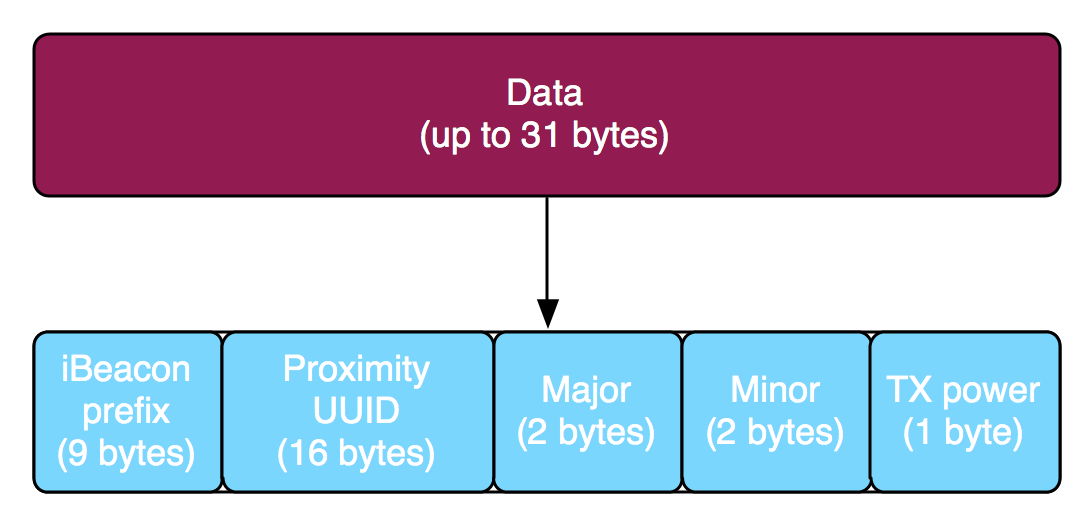
\includegraphics[scale=0.5]{img/ibeacon-advertisement}	
\end{center}

\begin{itemize}
	\item The \textbf{UUID} usually identifies the owner of the beacons (be it a company, or a store);
	\item The \textbf{major} number is used to group a related set of beacons. In our implementation, each beacon in the same classroom has the same major number;
	\item The \textbf{minor} number is used to identify individual beacons;
	\item The \textbf{TX Power} field is the strength of the signal measured at 1 meter from the device, and can be used to determine the distance from the beacon.
\end{itemize}

iOS provides built in capabilities to read the fields of an iBeacon advertisement through its CoreLocationFramework.